\setcounter{section}{0}
\chapter{VẬT LÝ NHIỆT}
\section{SỰ CHUYỂN THỂ}
\subsection{LÝ THUYẾT TRỌNG TÂM}
\begin{tomtat}
\subsubsection{Mô hình động học phân tử về cấu tạo chất}
\begin{boxdn}
	Mô hình động học phân tử về cấu tạo chất có những nội dung cơ bản sau:
	\begin{enumerate}[label=\arabic*.]
		\item Các chất được cấu tạo từ các hạt riêng biệt gọi là phân tử.
		\item Các phân tử chuyển động hỗn loạn, không ngừng. Nhiệt độ của vật càng cao thì tốc độ chuyển động của các phân tử cấu tạo nên vật càng lớn.
		\item Giữa các phân tử có lực hút và đẩy gọi chung là lực liên kết phân tử.
	\end{enumerate}
\end{boxdn}
\subsubsection{Cấu trúc của chất rắn, lỏng, khí}
\paragraph{Phân biệt cấu trúc của chất rắn, lỏng, khí}
\begin{center}
	\begin{tabular}{|p{4cm}|p{4cm}|p{4cm}|p{4cm}|}
		\hline
		\rowcolor{blue!25!white}
		\thead{Đặc điểm}&\thead{Thể rắn} &\thead{Thể lỏng}&\thead{Thể khí}\\
		\hline
		Khoảng cách giữa các phân tử & Rất gần nhau (cỡ kích thước phân tử) & Xa nhau & Rất xa nhau (gấp hàng chục lần kích thước phân tử)\\
		\hline
		Lực tương tác phân tử & Rất mạnh & Nhỏ hơn trong chất rắn & Rất yếu\\
		\hline
		Sự sắp xếp của các phân tử & Trật tự & Kém trật tự hơn & Không có trật tự\\
		\hline
		Chuyển động của các phân tử & Chỉ dao động quanh vị trí cân bằng cố định & Dao động quanh vị trí cân bằng luôn luôn thay đổi & Chuyển động hỗn loạn \\
		\hline
		Hình dạng & Hình dạng riêng xác định & Có hình dạng của bình chứa & Có hình dạng của bính chứa\\
		\hline
		Thể tích & Xác định & Xác định & Chiếm toàn bộ thể tích bình chứa\\
		\hline
	\end{tabular}
\end{center}
\paragraph{Chất rắn kết tinh và chất rắn vô định hình}
\begin{dn}
	\begin{itemize}
		\item \textbf{Chất rắn kết tinh} là chất mà các hạt (phân tử, nguyên tử, ion) cấu tạo nên nó ở thể rắn, liên kết với nhau một cách chặt chẽ, sắp xếp theo một trật tự hình học xác định tạo thành các mạng tinh thể.
	\end{itemize}
\end{dn}
\textit{\textbf{Ví dụ:}} muối ăn, thạch anh, kim cương, nước đá, \dots
	\begin{center}
		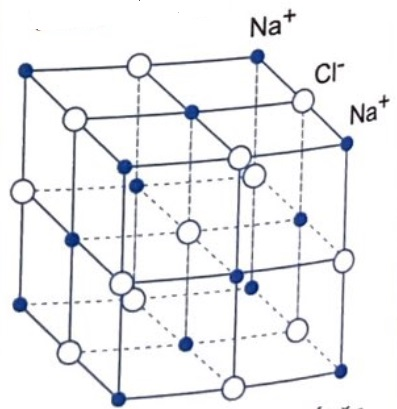
\includegraphics[width=0.2\linewidth]{figs/VN12-Y24-PH-SYL-001-3}
		\captionof{figure}{Cấu trúc tinh thể muối ăn}
	\end{center}
	\begin{dn}
		\begin{itemize}
		\item \textbf{Chất rắn vô định hình} là chất ở thể rắn mà các hạt tạo nên nó không tạo thành mạng tinh thể.\\
	\end{itemize}
	\end{dn}
	\textbf{\textit{Ví dụ:}} thuỷ tinh, nhựa đường, sôcôla, \dots
\subsubsection{Sự chuyển thể}
\begin{dn}
	Khi các điều kiện như nhiệt độ, áp suất thay đổi, chất có thể chuyển từ thể này sang thể khác.
	\begin{itemize}
		\item Quá trình chuyển từ thể rắn sang thể lỏng của các chất được gọi là \textit{sự nóng chảy}. Quá trình ngược lại gọi là sự đông đặc.
		\item Quá trình chuyển từ thể lỏng sang thể khí (hơi) của các chất được gọi là \textit{sự hoá hơi}. Quá trình chuyển ngược lại gọi là sự ngưng tụ.
		\item Trong một số điều kiện, chất rắn có thể chuyển sang thể khí (hơi). Quá trình này gọi là sự thăng hoa. Quá trình ngược lại gọi là sự ngưng kết.\\
	\end{itemize}
\end{dn}
	\textit{\textbf{Ví dụ:}} Sự thăng hoa dễ dàng của băng phiến ở nhiệt độ thường. Sự ngưng kết của hơi nước trong không khí tạo thành sương muối.
	\begin{center}
		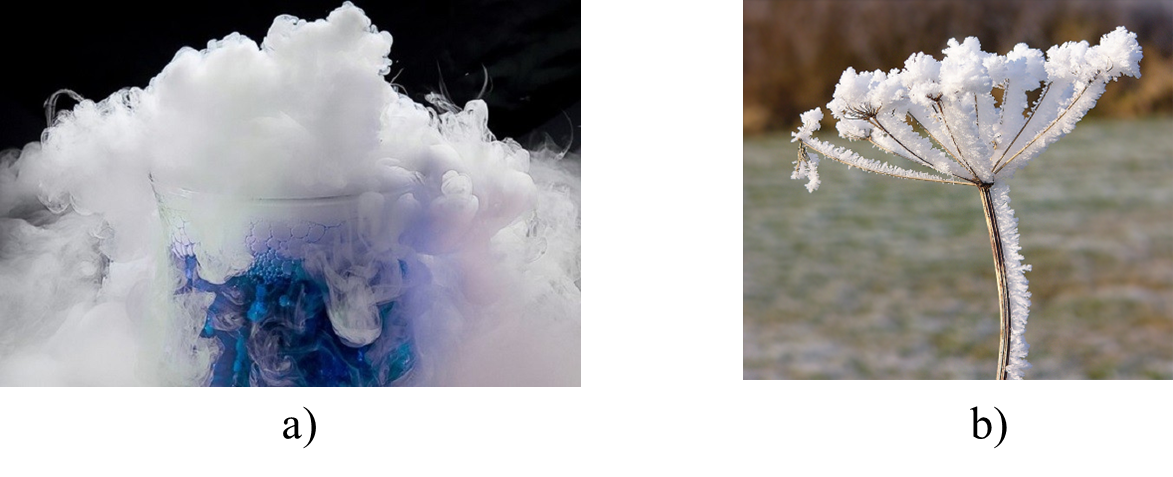
\includegraphics[width=0.7\linewidth]{figs/VN12-Y24-PH-SYL-001-7}
		\captionof{figure}{a) Đá khô thăng hoa; b) Sương muối}
	\end{center}

\begin{center}
	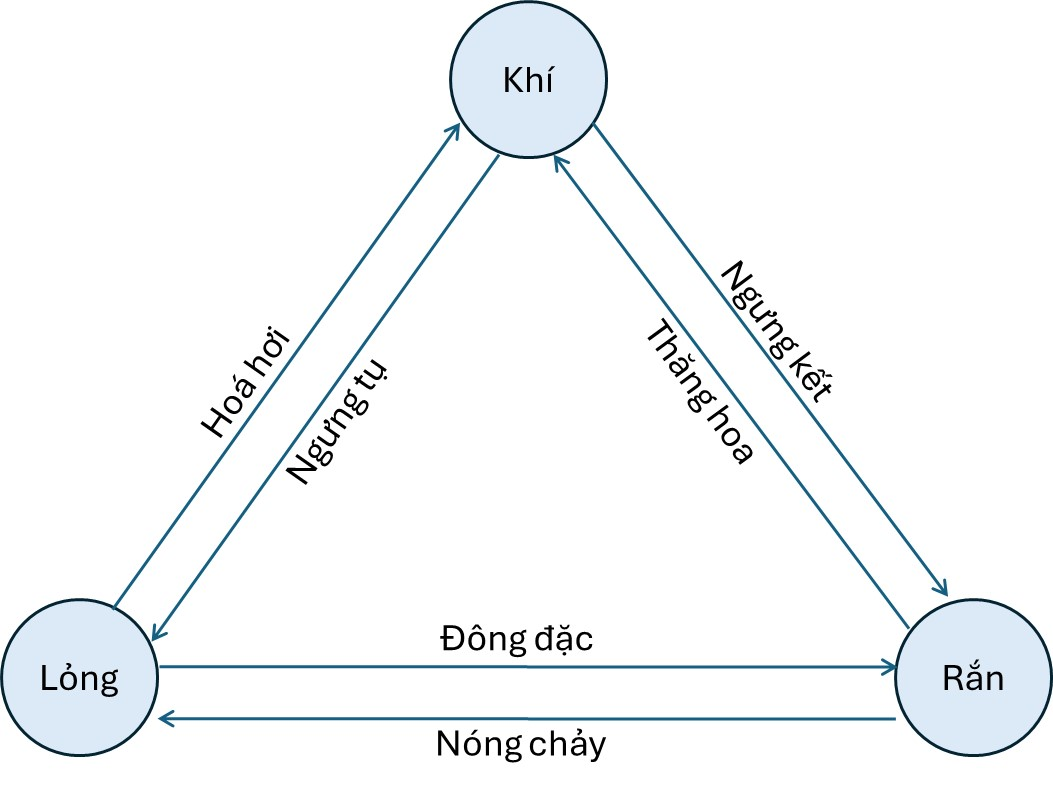
\includegraphics[width=0.5\linewidth]{figs/VN12-Y24-PH-SYL-001-4}
	\captionof{figure}{Sơ đồ các hình thức chuyển thể}
\end{center}
\paragraph{Sự nóng chảy}
\begin{dn}
	Khi đun nóng đến một nhiệt độ nào đó, vật rắn bắt đầu chuyển trạng thái từ rắn sang lỏng (sự nóng chảy). Chất rắn kết tinh có nhiệt độ nóng chảy xác định (ở một áp suất cụ thể). Chất rắn vô định hình không có nhiệt độ nóng chảy xác định.\\
\end{dn}
	\textbf{\textit{Ví dụ:}}
	\begin{itemize}
		\item Khi nung nóng nước đá ở áp suất tiêu chuẩn, nhiệt độ nước đá tăng dần. Khi đạt đến $\SI{0}{\celsius}$, nước đá bắt đầu tan và trong suốt quá trình hoá lỏng nhiệt độ của nước đá không đổi. Nước đá là chất rắn kết tinh.
		\item Khi nung nóng thỏi sôcôla, thỏi sôcôla mềm đi và chuyển dần sang thể lỏng, trong quá trình này nhiệt độ của thỏi sôcôla vẫn tăng liên tục. Thỏi sôcôla là chất rắn vô định hình.
	\end{itemize}
	\begin{center}
		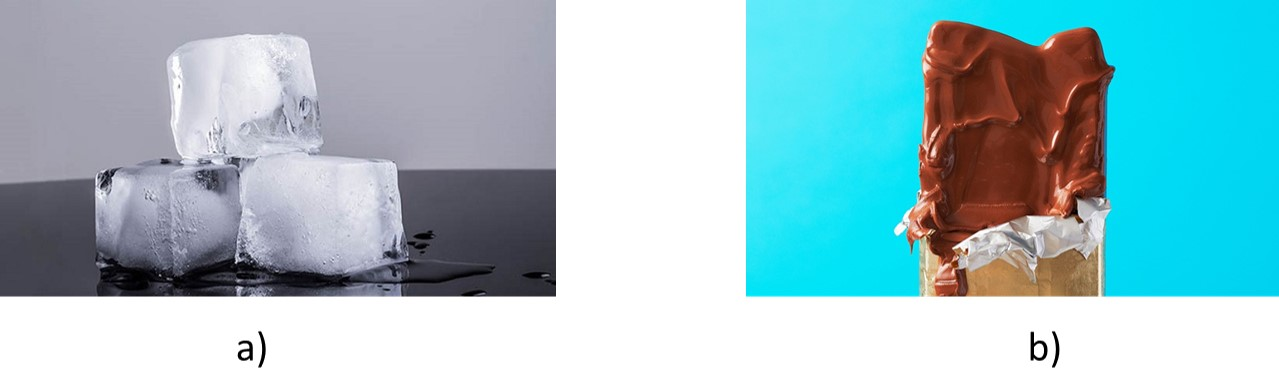
\includegraphics[width=0.6\linewidth]{figs/VN12-Y24-PH-SYL-001-5}
		\captionof{figure}{a) Nước đá đang tan; b) Thanh sôcôla đang nóng chảy}
	\end{center}
\paragraph{Sự hoá hơi}
\begin{dn}
	\begin{itemize}
		\item \textbf{Sự bay hơi}\\
		Sự bay hơi là sự hoá hơi xảy ra \textbf{trên bề mặt chất lỏng}. Sự bay hơi xảy ra ở \textbf{nhiệt độ bất kì}.\\
		Tốc độ bay hơi của chất lỏng càng nhanh nếu diện tích mặt thoáng càng lớn, tốc độ gió càng lớn, nhiệt độ càng cao, và độ ẩm không khí càng thấp.
		\item \textbf{Sự sôi}\\
		Sự sôi là sự hoá hơi xảy ra \textbf{bên trong và trên bề mặt chất lỏng}. Sự sôi xảy ra ở \textbf{nhiệt độ sôi}.\\
		Nhiệt độ sôi của chất lỏng phụ thuộc áp suất khí trên mặt thoáng và bản chất của chất lỏng. Trong suốt thời gian sôi, nhiệt độ của chất lỏng không thay đổi.
	\end{itemize}
\end{dn}
\begin{center}
	
	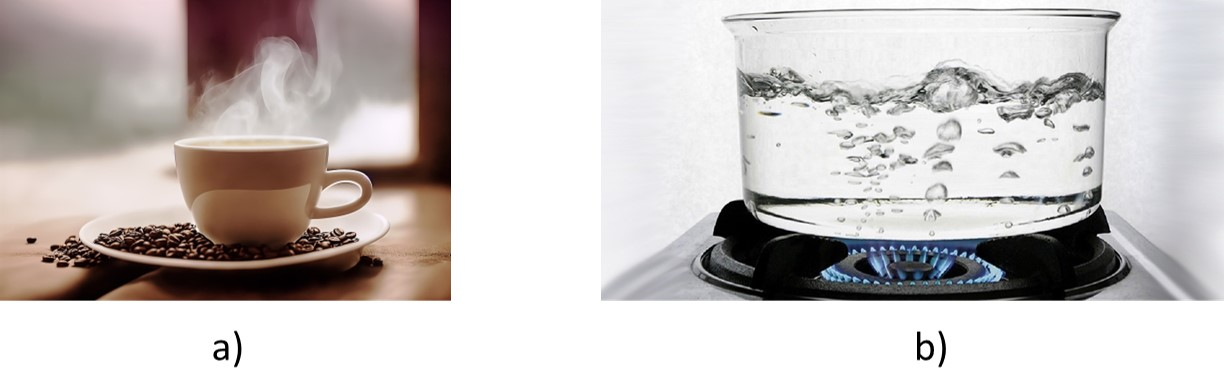
\includegraphics[width=0.65\linewidth]{figs/VN12-Y24-PH-SYL-001-6}
	\captionof{figure}{a) Nước bay hơi trên mặt thoáng của tách cà phê; b) Nước đang sôi}
\end{center}
\end{tomtat}
\subsection{VÍ DỤ MINH HOẠ}
\begin{dang}{Sử dụng mô hình động học phân tử, nêu được sơ lược cấu trúc của chất rắn, chất lỏng, chất khí}
\end{dang}
\begin{vd}
	Năm 1827, khi làm thí nghiệm quan sát các hạt phấn hoa rất nhỏ trong nước bằng kính hiển vi, Brown thấy chúng chuyển động hỗn loạn, không ngừng. Chuyển động này được gọi là chuyển động Brown.\\
	\begin{center}
		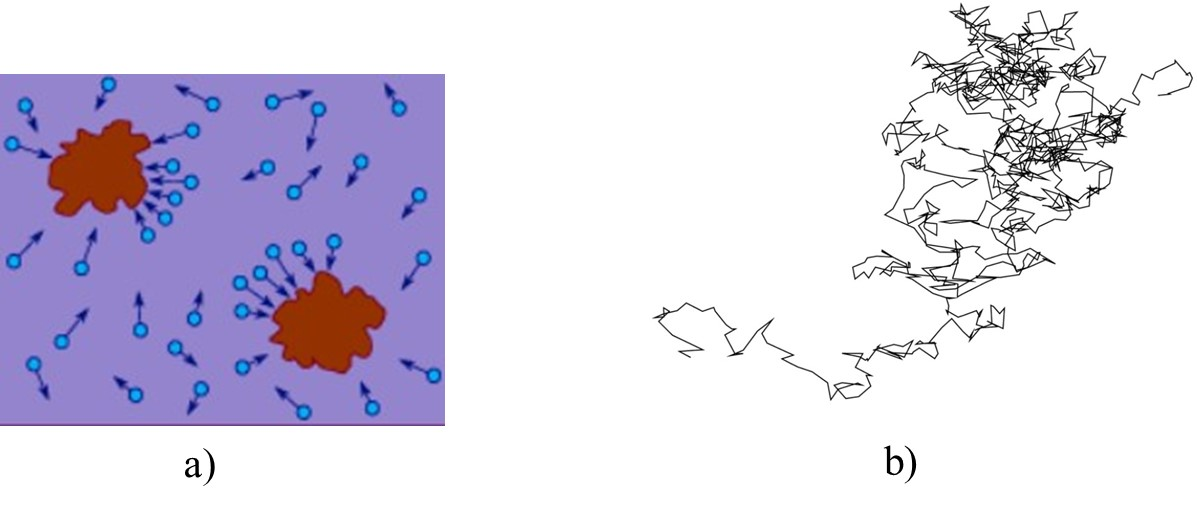
\includegraphics[width=0.6\linewidth]{figs/VN12-Y24-PH-SYL-001-1}
		\captionof{figure}{a) Mô phỏng sự va chạm giữa các phân tử nước với các hạt phấn hoa; b) Quỹ đạo chuyển động của hạt phấn hoa}
	\end{center}
	\begin{enumerate}[label=\alph*)]
		\item Tại sao thí nghiệm của Brown được gọi là một trong những thí nghiệm chứng tỏ các phân tử chuyển động hỗn loạn không ngừng?
		\item Làm thế nào để với thí nghiệm của Brown có thể chứng tỏ được khi nhiệt độ của nước càng cao thì các phân tử nước chuyển động càng nhanh?
	\end{enumerate}
	\loigiai{
		\begin{enumerate}[label=\alph*)]
			\item Thông qua việc quan sát hạt phấn hoa trong nước, Brown nhận thấy rằng các hạt phấn hoa lắc lư không ngừng và quỹ đạo chuyển động của hạt phấn hoa hỗn loạn. Mà chuyển động của hạt phấn hoa là do sự va chạm  giữa các phân tử nước với hạt phấn hoa gây ra. Điều này chứng tỏ rằng chuyển động của các phân tử nước cũng hỗn loạn, không ngừng.
			\item Để với thí nghiệm của Brown có thể chứng tỏ được khi nhiệt độ của nước càng cao thì các phân tử nước chuyển động càng nhanh thì chúng ta có thể đun nóng nước rồi quan sát sự thay đổi tốc độ chuyển động của hạt phấn hoa.
	\end{enumerate}}
\end{vd}
\begin{vd}
	Hãy giải thích đặc điểm sau đây của thể khí, thể rắn, thể lỏng.
	\begin{enumerate}[label=\alph*)]
		\item Chất khí không có hình dạng và thể tích riêng, luôn chiếm toàn bộ thể tích bình chứa và có thể nén được dễ dàng.
		\item Vật ở thể rắn có thể tích và hình dạng riêng, rất khó nén.
		\item Vật ở thể lỏng có thể tích riêng nhưng không có hình dạng riêng.
	\end{enumerate}
	\loigiai{
		\begin{enumerate}[label=\alph*)]
			\item Ở thể khí, các phân tử ở xa nhau (khoảng cách giữa các phân tử lớn gấp hàng chục lần kích thước phân tử). Lực tương tác giữa các phân tử rất yếu (trừ trường hợp chúng va chạm nhau) nên các phân tử chuyển động hoàn toàn hỗn loạn. Do đó, khối chất khí không có hình dạng và thể tích riêng mà có hình dạng và thể tích của bình chứa nó.
			\item Ở thể rắn, các phân tử rất gần nhau (khoảng cách giữa các phân tử cỡ kích thước phân tử) và các phân tử sắp xếp có trật tự, chặt chẽ. Lực tương tác giữa các phân tử rất mạnh, giữ cho chúng không di chuyển tự do mà chỉ có thể dao động quanh vị trí cân bằng xác định. Do đó, vật rắn luôn có thể tích và hình dạng riêng xác định, đồng thời rất khó nén.
			\item Khoảng cách giữa các phân tử trong chất lỏng lớn hơn khoảng cách giữa các phân tử trong chất rắn và nhỏ hơn khoảng cách giữa các phân tử trong chất khí. Lực tương tác giữa các phân tử ở thể lỏng lớn hơn lực tương tác giữa các phân tử ở thể khí nên giữ các phân tử không bị phân tán ra xa nhau, do đó chất lỏng có thể tích riêng xác định. Lực tương tác này chưa đủ lớn như trong thể rắn nên các phân tử ở thể lỏng cũng dao động quanh vị trí cân bằng nhưng các vị trí cân bằng này luôn luôn thay đổi. Do đó, khối chất lỏng không có hình dạng riêng xác định mà có hình dạng của bình chứa nó.
	\end{enumerate}}
\end{vd}

\begin{dang}{Giải thích được sơ lược một số hiện tượng vật lí liên quan đến sự chuyển thể: sự nóng chảy, sự hoá hơi}
\end{dang}
%\setcounter{vd}{0}
\begin{vd}
	Vận dụng mô hình động học phân tử, em hãy giải thích nguyên nhân gây ra sự nóng chảy của chất rắn kết tinh.
	\loigiai{
		Ở áp suất không đổi, các phân tử ở thể rắn liên kết chặt chẽ với nhau, chúng dao động quanh các vị trí cân bằng xác định. Khi nung nóng chất rắn kết tinh, các phân tử được cung cấp nhiệt năng làm tốc độ chuyển động nhiệt của nó tăng lên, mức độ trật tự trong cấu trúc của các hạt giảm đi.  Điều này dẫn đến khoảng cách trung bình giữa các phân tử tăng.\\
		Nhiệt độ của vật rắn tăng đến một giá trị nào đó thì một số phân tử thắng được lực liên kết với các phân tử xung quanh và thoát khỏi liên kết với chúng, đó là sự khởi đầu của quá trình nóng chảy. Từ lúc này, vật rắn nhận nhiệt lượng để tiếp tục phá vỡ các liên kết tinh thể. Khi trật tự của tinh thể bị phá vỡ hoàn toàn thì quá trình nóng chảy kết thúc, vật rắn chuyển thành khối chất lỏng.
	}
\end{vd}
\begin{vd}
	Vận dụng mô hình động học phân tử, em hãy giải tích nguyên nhân gây ra sự bay hơi và sự sôi.

\loigiai{\textbf{Giải thích sự bay hơi:}\\
		Các phân tử ở bề mặt chất lỏng tham gia chuyển động nhiệt, trong đó có những phân tử chuyển động hướng ra ngoài chất lỏng. Đồng thời, các phân tử có thể truyền năng lượng cho nhau thông qua quá trình va chạm. Do đó, một số phân tử ở gần mặt thoáng của chất lỏng có động năng đủ lớn để thắng lực liên kết của các phân tử chất lỏng khác thì thoát được ra khỏi mặt thoáng của chất lỏng trở thành các phân tử ở thể hơi.\\
		\textbf{Giải thích sự sôi:}\\
		Khi chất lỏng đến nhiệt độ sôi, do tiếp tục được cung cấp nhiệt nên các phân tử chất lỏng chuyển động nhiệt mạnh hơn, làm phá vỡ sự liên kết giữa các phân tử chất lỏng với nhau. Khi đó các bọt chứa không khí và hơi nước nổi lên trong lòng nước càng ngày càng nhiều, càng nổi lên trên thể tích các bọt khí này càng tăng, tới mặt thoáng thì vỡ, không khí và hơi nước thoát ra ngoài khí quyển.

}
\end{vd}


\subsection{BÀI TẬP TRẮC NGHIỆM}

\Opensolutionfile{ans}[ans/G12Y24B1TN]
\begin{ex}
Chuyển động của các nguyên tử, phân tử trong mô hình động học phân tử được gọi là chuyển động
\choice
{chuyển động cơ}
{\True chuyển động nhiệt}
{chuyển động tròn}
{chuyển động đều}
\loigiai{ }
\end{ex}

%==============================================
\begin{ex}

Chọn phát biểu \textbf{đúng} về lực tương tác giữa các phân tử.
\choice
{\True Giữa các phân tử có cả lực hút và lực đẩy}
{ Giữa các phân tử chỉ có lực hút hoặc lực đẩy}
{ Giữa các phân tử chỉ có lực đẩy}
{ Giữa các phân tử chỉ có lực hút}
\loigiai{ }
\end{ex}

%==============================================
\begin{ex}
Khi khoảng cách giữa các phân tử rất nhỏ, thì giữa các phân tử
\choice
{ chỉ có lực hút}
{ chỉ có lực đẩy}
{\True có cả lực hút và lực đẩy, nhưng lực đẩy lớn hơn lực hút}
{ có cả lực hút và lực đẩy, nhưng lực đẩy nhỏ hơn lực hút}
\loigiai{ }
\end{ex}


%==============================================
\begin{ex}
Mục đích của thí nghiệm Brown là
\choice
{ quan sát hạt phấn hoa bằng kính hiển vi}
{\True quan sát chuyển động của hạt phấn hoa trong nước bằng kính hiển vi}
{ quan sát cánh hoa trong nước bằng kính hiển vi}
{ quan sát chuyển động của cánh hoa}
\loigiai{ }
\end{ex}


%==============================================
\begin{ex} 
Trong thí nghiệm của Brown các hạt phấn hoa chuyển động hỗn độn, không ngừng vì
\choice
{ giữa các hạt phấn hoa có lực tương tác hút và đẩy}
{ các hạt phấn hoa là các thực thể sống}
{\True các phân tử nước chuyển động không ngừng, va chạm vào chúng từ mọi phía}
{ các hạt phấn hoa có thể dao động tự do quanh vị trí cân bằng}
\loigiai{ }
\end{ex}


%==============================================
\begin{ex}
Chọn câu trả lời \textbf{đúng nhất}. \\
Các chất có thể tồn tại ở những thể nào?
\choice
{ Thể rắn, thể lỏng, thể khí hoặc chân không}
{\True Thể rắn, thể lỏng hoặc thể khí}
{ Thể rắn và thể hơi}
{ Thể rắn và thế lỏng}
\loigiai{ }
\end{ex}


%==============================================
\begin{ex}
Đặc điểm nào sau đây là phù hợp với chất rắn?
\choice
{\True Có lực tương tác giữa các phân tử rất mạnh}
{ Có lực tương tác giữa các phân tử rất yếu}
{ Không có hình dạng xác định}
{ Không có thể tích riêng xác định}
\loigiai{ }
\end{ex}


%==============================================
\begin{ex}
Phát biểu nào dưới đây là đúng khi nói về những đặc điểm của chất rắn?
\choice
{ Có khối lượng, hình dạng xác định, không có thể tích xác định}
{ Có khối lượng xác định, hình dạng và thể tích không xác định}
{\True Có khối lượng, hình dạng, thể tích xác định}
{ Có khối lượng và thể tích xác định, hình dạng không xác định}
\loigiai{ }
\end{ex}


%==============================================
\begin{ex}
Người ta có thể phân loại chất rắn một cách tổng quát theo cách nào sau đây?
\choice
{ Chất rắn đơn tinh thể và chất rắn vô định hình}
{\True Chất rắn kết tinh và chất rắn vô định hình}
{ Chất rắn đa tinh thể và chất rắn vô định hình}
{ Chất rắn đơn tinh thể và chất rắn đa tinh thể}
\loigiai{ }
\end{ex}


%==============================================
\begin{ex} 
Đặc điểm nào sau đây là đặc điểm cấu trúc phân tử ở thể lỏng?
\choice
{ Khoảng cách giữa các phân tử rất lớn so với kích thước của chúng}
{\True Lực tương tác phân tử yếu hơn lực tương tác phân tử ở thể rắn}
{ Không có thể tích và hình dạng riêng xác định}
{ Các phân tử dao động xung quanh vị trí cân bằng xác định}
\loigiai{ }
\end{ex}


%==============================================
\begin{ex} 
Trong chuyển động nhiệt, các phân tử chất lỏng
\choice
{ dao động quanh vị trí cân bằng xác định}
{ chuyển động hỗn loạn quanh vị trí cân bằng xác định}
{ chuyển động hỗn loạn}
{\True dao động quanh vị trí cân bằng nhưng những vị trí này không cố định mà luôn thay đổi}
\loigiai{ }
\end{ex}


%==============================================
\begin{ex}
Chất lỏng có thể tích xác định, nhưng hình dạng không xác định là do trong chất lỏng
\choice
{ lực liên kết giữa các phân tử chất lỏng là rất lớn, các phân tử chỉ dao động không ngừng quanh một vị trí xác định}
{ lực liên kết giữa các phân tử chất lỏng là rất yếu, các phân tử dao động tự do về mọi phía}
{\True lực liên kết giữa các phân tử chất lỏng là yếu hơn chất rắn, các phân tử dao động tương đối tự do hơn so với trong chất rắn}
{ Tất cả các phương án đưa ra đều sai}
\loigiai{ }
\end{ex}


%==============================================
\begin{ex} 
Các phân tử khí chuyển động hỗn loạn, không ngừng vì
\choice
{ phân tử khí không có khối lượng}
{ khoảng cách giữa các phân tử khí quá gần nhau}
{\True lực tương tác giữa các phân tử quá nhỏ}
{ các phân tử khí luôn đẩy nhau}
\loigiai{ }
\end{ex}


%==============================================
\begin{ex}
Tính chất nào sau đây \textbf{không phải} là tính chất của chất ở thể khí?
\choice
{\True Có hình dạng và thể tích riêng}
{ Có các phân tử chuyển động hoàn toàn hỗn độn}
{ Có thể nén được dễ dàng}
{ Có lực tương tác phân tử nhỏ hơn lực tương tác phân tử ở thể rắn và thể lỏng}
\loigiai{ }
\end{ex}


%==============================================
\begin{ex}
Chất khí không có hình dạng và thể tích riêng là vì
\choice
{ khoảng cách giữa các phân tử rất gần, lực tương tác giữa các phân tử chất khí rất mạnh}
{ khoảng cách giữa các phân tử rất gần, lực tương tác giữa các phân tử chất khí rất yếu}
{ khoảng cách giữa các phân tử rất xa, lực tương tác giữa các phân tử chất khí rất mạnh}
{\True khoảng cách giữa các phân tử rất xa, lực tương tác giữa các phân tử chất khí rất yếu}
\loigiai{ }
\end{ex}


%==============================================
\begin{ex}
Khi mở nắp lọ nước hoa, ta có thể ngửi thấy mùi thơm tràn ngập trong phòng. Điều này thể hiện tính chất nào của chất khí?
\choice
{ Dễ dàng nén được}
{ Có khối lượng xác định}
{\True Có thể khuếch tán trong không gian theo mọi hướng}
{ Không chảy được}
\loigiai{ }
\end{ex}


%==============================================
\begin{ex}
Sự nóng chảy là
\choice
{\True sự chuyển thế từ rắn sang lỏng}
{ sự chuyển thể từ rắn sang khí}
{ sự chuyển thể từ lỏng sang rắn}
{ sự chuyển thể từ lỏng sang khí}
\loigiai{ }
\end{ex}


%==============================================
\begin{ex}
Sự đông đặc là
\choice
{ sự chuyển thế từ rắn sang lỏng}
{ sự chuyển thể từ rắn sang khí}
{\True sự chuyển thể từ lỏng sang rắn}
{ sự chuyển thể từ lỏng sang khí}
\loigiai{ }
\end{ex}
%==============================================
\begin{ex}
Sự bay hơi là
\choice
{ sự chuyển thế từ rắn sang lỏng}
{ sự chuyển thể từ rắn sang khí}
{ sự chuyển thể từ lỏng sang rắn}
{\True sự chuyển thể từ lỏng sang khí}
\loigiai{ }
\end{ex}
%==============================================
\begin{ex}
Khi quan sát sự nóng chảy của nước đá, trong suốt thời gian nóng chảy thì
\choice
{ nhiệt độ của nước đá tăng}
{ nhiệt độ của nước đá giảm}
{\True nhiệt  độ của nước đá không đổi}
{ nhiệt độ của nước đá ban đầu tăng và sau đó giảm}
\loigiai{ }
\end{ex}
%==============================================
\begin{ex}
Phát biểu nào sau đây về tính chất của chất rắn kết tinh và chất rắn vô định hình là \textbf{đúng}?
\choice
{ Chất rắn kết tinh và chất rắn vô định hình đều có nhiệt độ nóng chảy xác định}
{ Chất rắn kết tinh không có nhiệt độ nóng chảy xác định, chất rắn vô định hình có nhiệt độ nóng chảy xác định}
{\True Chất rắn kết tinh có nhiệt độ nóng chảy xác định, chất rắn vô định hình không có nhiệt độ nóng chảy xác định}
{ Chất rắn kết tinh và chất rắn vô định hình đều không có nhiệt độ nóng chảy xác định}
\loigiai{ }
\end{ex}
%==============================================
\begin{ex}
Một vật rắn khi bị nung nóng thì mềm dần. Đó là
\choice
{ chất rắn kết tinh}
{ chất rắn đơn tinh thể}
{ chất rắn đa tinh thể}
{\True chất rắn vô định hình}
\loigiai{ }
\end{ex}
%==============================================
\begin{ex}
Trường hợp nào sau đây không liên quan đến sự nóng chảy và đông đặc?
	\begin{center}
		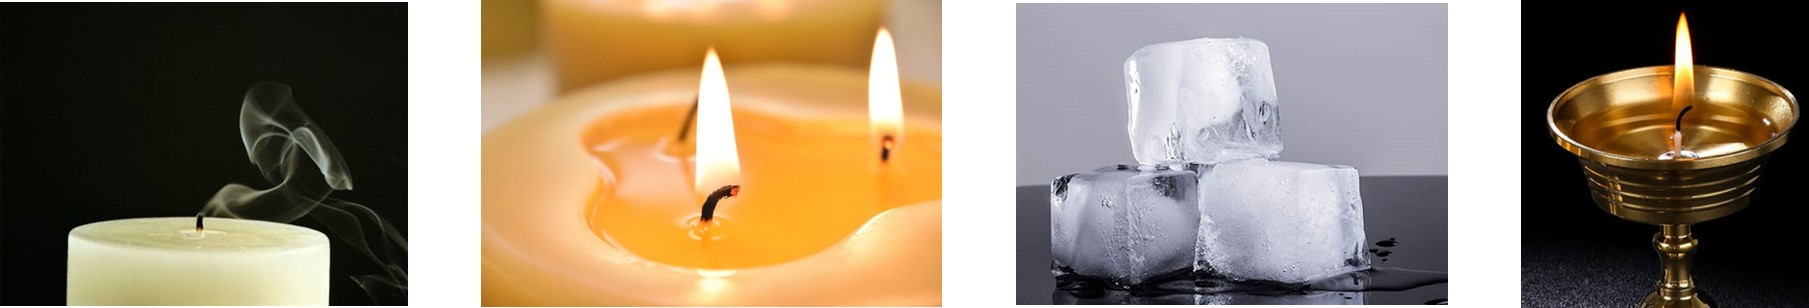
\includegraphics[width=0.45\linewidth]{figs/VN12-Y24-PH-SYL-001P-2}
	\end{center}
\choice
{ Ngọn nến vừa tắt}
{ Ngọn nến đang cháy}
{ Nước đá vừa lấy ra khỏi tủ lạnh}
{\True Ngọn đèn dầu đang cháy}
\loigiai{ }
\end{ex}
%==============================================
\begin{ex}
Sự bay hơi diễn ra càng nhanh hơn khi
\choice
{ nhiệt độ càng thấp}
{\True tốc độ gió càng lớn}
{ lượng chất lỏng càng nhiều}
{ diện tích mặt thoáng càng hẹp}
\loigiai{ }
\end{ex}
%==============================================
\begin{ex}
Một ấm nước đang sôi, nếu tiếp tục đun thì
\choice
{ nhiệt độ nước trong ấm giảm xuống}
{ nước trong ấm không bay hơi nữa}
{ nhiệt độ nước trong ấm vẫn tiếp tục tăng}
{\True nước trong ấm bay hơi nhiều hơn và cạn dần}
\loigiai{ }
\end{ex}
%==============================================
\begin{ex}
Phát biểu nào sau đây là \textbf{không đúng} về sự bay hơi?
\choice
{ Sự bay hơi là quá trình chuyển từ thể lỏng sang thể khí xảy ra ở bề mặt chất lỏng}
{\True Sự bay hơi là quá trình chuyển từ thể lỏng sang thể khí xảy ra ở cả bên trong và trên bề mặt chất lỏng}
{ Sự bay hơi của chất lỏng xảy ra ở nhiệt độ bất kì}
{ Sự ngưng tụ luôn kèm theo sự bay hơi}
\loigiai{ }
\end{ex}
%==============================================
\begin{ex}
Sự sôi xảy ra ở
\choice
{ nhiệt độ trên $\SI{100}{\celsius}$}
{ $\SI{100}{\celsius}$}
{\True nhiệt độ sôi}
{ dưới $\SI{100}{\celsius}$}
\loigiai{ }
\end{ex}
%==============================================
\begin{ex}
Trong các trường hợp dưới đây, trường hợp nào liên quan đến sự bay hơi?
\choice
{ Kính cửa sổ bị mờ đi trong những ngày đông giá lạnh}
{\True Dầu trong đèn bị khô cạn dù không sử dụng}
{ Miếng bơ để bên ngoài tủ lạnh sau một thời gian bị chảy lỏng}
{ Đưa nước vào trong tủ lạnh để làm đá}
\loigiai{ }
\end{ex}
%==============================================
\begin{ex}
Tại sao quả bóng bay dù buộc chặt để lâu ngày vẫn bị xẹp?
\choice
{ Vì khi mới thổi, không khí từ miệng vào bóng còn nóng, sau đó lạnh dần nên co lại}
{ Vì cao su là chất đàn hồi nên sau khi bị thổi căng nó tự động co lại}
{ Vì không khí nhẹ nên có thể chui qua chỗ buộc ra ngoài}
{\True Vì giữa các phân tử của chất làm vỏ bóng có khoảng cách nên các phân tử không khí có thể chui qua đó và thoát ra ngoài}
\loigiai{ }
\end{ex}
%==============================================
\begin{ex}
Hãy chọn phương án \textbf{sai}.\\
Cùng một khối lượng của một chất nhưng khi ở các thể khác nhau thì sẽ khác nhau
\choice
{ Thể tích}
{ Khối lượng riêng}
{\True Kích thước của các nguyên tử}
{ Trật tự của các nguyên tử}
\loigiai{ }
\end{ex}
%==============================================
\begin{ex}
Các nguyên tử trong một miếng sắt có tính chất nào sau đây?
\choice
{ Khi nhiệt độ tăng thì nở ra}
{ Khi nhiệt độ giảm thì co lại}
{\True Đứng rất gần nhau}
{ Đứng xa nhau}
\loigiai{ }
\end{ex}
%==============================================
\begin{ex}
Trong các chất sau, chất nào \textbf{không phải} là chất rắn kết tinh?
\choice
{ Muối ăn}
{\True Thuỷ tinh}
{ Kim cương}
{ Thạch anh}
\loigiai{ }
\end{ex}
%==============================================
\begin{ex}
Chất rắn nào dưới đây không phải là chất rắn vô định hình?
\choice
{\True Thạch anh}
{ Thuỷ tinh}
{ Sáp}
{ Cao su}
\loigiai{ }
\end{ex}
%==============================================
\begin{ex}
Chất rắn nào dưới đây là chất rắn vô định hình?
\choice
{ Muối ăn}
{ Kim loại}
{ Thạch anh}
{\True Nhựa đường}
\loigiai{ }
\end{ex}
%==============================================
\begin{ex}
Ở điều kiện thường, iode là chất rắn dạng tinh thể màu đen tím. Khi đun nóng, iode có sự thăng hoa.\\
Vậy sự thăng hoa của iode là sự chuyển trạng thái từ thể
\choice
{\True rắn sang khí}
{ rắn sang lỏng}
{ lỏng sang rắn}
{ khí sang rắn}
\loigiai{ }
\end{ex}
%==============================================
\begin{ex}
Cho đồ thị biểu diễn sự thay đổi nhiệt độ theo thời gian của nước đá như hình vẽ. Nước đá tan trong khoảng thời gian nào?
\begin{center}
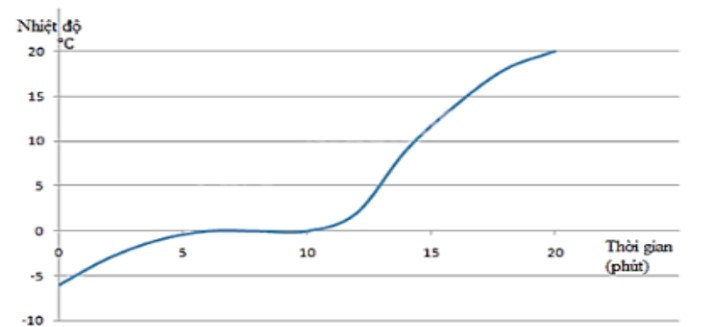
\includegraphics[width=0.6\linewidth]{figs/VN12-Y24-PH-SYL-001P-1}
\end{center}
\choice
{\True Từ phút thứ 6 đến phút thứ 10}
{ Từ phút thứ 10 trở đi}
{ Từ 0 đến phút thứ 6}
{ Từ phút thứ 10 đến phút thứ 15}
\loigiai{ }
\end{ex}
%==============================================
\begin{ex}
Người ta không thể luộc trứng chín ở núi cao vì
\choice
{\True áp suất trên núi thấp hơn áp suất chuẩn $\left(\SI{1}{atm}\right)$ nên nước sôi ở nhiệt độ thấp hơn $\SI{100}{\celsius}$}
{ áp suất trên núi cao hơn áp suất chuẩn $\left(\SI{1}{atm}\right)$ nên nước sôi ở nhiệt độ thấp hơn $\SI{100}{\celsius}$}
{ áp suất trên núi thấp hơn áp suất chuẩn $\left(\SI{1}{atm}\right)$ nên nước sôi ở nhiệt độ cao hơn $\SI{100}{\celsius}$}
{ áp suất trên núi cao hơn áp suất chuẩn $\left(\SI{1}{atm}\right)$ nên nước sôi ở nhiệt độ cao hơn $\SI{100}{\celsius}$}
\loigiai{ }
\end{ex}
%==============================================
\begin{ex}
Thuỷ ngân có nhiệt độ nóng chảy là $\SI{-39}{\celsius}$ và nhiệt độ sôi là $\SI{357}{\celsius}$. Khi ở trong phòng có nhiệt độ $\SI{30}{\celsius}$ thì thuỷ ngân
\choice
{chỉ tồn tại ở thể lỏng}
{ chỉ tồn tại ở thể hơi}
{\True  tồn tại ở cả thể lỏng và thể hơi}
{ tồn tại ở cả thể rắn, lỏng và hơi}
\loigiai{ }
\end{ex}
%==============================================
\begin{ex}
Tại sao khi cầm vào vỏ bình ga mini đang sử dụng ta thường thấy có một lớp nước rất
mỏng trên đó?
\choice
{ Do hơi nước từ tay ta bốc ra}
{ Nước từ trong bình ga thấm ra}
{\True Do vỏ bình ga lạnh hơn nhiệt độ môi trường nên hơi nước trong không khí ngưng tụ trên đó}
{ Cả B và C đều đúng}
\loigiai{ }
\end{ex}
%==============================================
\begin{ex}
Ở nhiệt độ trong phòng, chỉ có thể có khí oxygen, không thể có oxygen lỏng vì
\choice
{ oxygen luôn là chất khí}
{\True nhiệt độ phòng cao hơn nhiệt độ sôi của oxygen}
{ nhiệt độ phòng thấp hơn nhiệt độ sôi của oxygen}
{ nhiệt độ trong phòng bằng nhiệt độ sôi của oxygen}
\loigiai{ }
\end{ex}

\Closesolutionfile{ans}

\subsection{TRẮC NGHIỆM ĐÚNG/SAI}
\Opensolutionfile{ans}[ans/G12Y24B1DS]
\setcounter{ex}{0}
% ===================================================================
\begin{ex}
	Nhận định các phát biểu sau đây về mô hình động học phân tử.
	\choiceTF[t]
	{\True Các chất được cấu tạo từ các hạt riêng biệt được gọi nguyên tử, phân tử}
	{Các nguyên tử, phân tử đứng sát nhau và giữa chúng không có khoảng cách}
	{\True Lực tương tác giữa các phân tử ở thể rắn lớn hơn lực tương tác giữa các phân tử ở thể lỏng và thể khí}
	{\True Các nguyên tử, phân tử chất lỏng dao động xung quanh các vị trí cân bằng không cố định}
	\loigiai{}
\end{ex}
% ===================================================================
\begin{ex}
		Nhận định các phát biểu về sự sôi.
	\choiceTF[t]
	{Nước chỉ sôi ở nhiệt độ $\SI{100}{\celsius}$}
	{\True Trong suốt thời gian sôi, nhiệt độ của nước không thay đổi}
	{Nước chỉ bay hơi ở nhiệt độ sôi}
	{\True Trong suốt thời gian sôi, nước vừa bay hơi tạo ra bọt khí và vừa bay hơi trên bề mặt\textbf{}}
	\loigiai{\begin{enumerate}[label=\alph*)]
			\item Sai. Nhiệt độ sôi của nước còn phụ thuộc vào áp suất nơi đun.
			\item Đúng.
			\item Sai. Nước bay hơi ở bất kì nhiệt độ nào.
			\item Đúng.
	\end{enumerate}}
\end{ex}
% ===================================================================
\begin{ex}
	Hình bên là đồ thị biểu diễn sự thay đổi nhiệt độ của nước theo thời gian đun.
	\begin{center}
		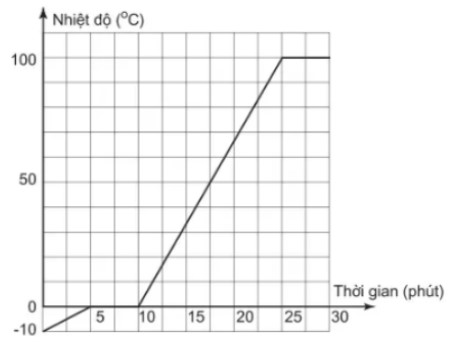
\includegraphics[width=0.45\linewidth]{figs/VN12-Y24-PH-SYL-001P-4}
	\end{center}
	\choiceTF[t]
	{\True Trong 5 phút đầu tiên, nước ở thể rắn}
	{\True Từ phút thứ 5 đến phút thứ 10 nước đá nóng chảy}
	{Từ phút thứ 10 đến phút thứ 25 nước không có sự bay hơi vì chưa đạt nhiệt độ sôi}
	{\True Nước được đun ở điều kiện tiêu chuẩn}
	\loigiai{\begin{enumerate}[label=\alph*)]
			\item Đúng.
			\item Đúng.
			\item Sai. Nước bay hơi ở bất kì nhiệt độ nào.
			\item Đúng. Đồ thị thể hiện quá trình nước sôi ở $\SI{100}{\celsius}$.
	\end{enumerate}}
\end{ex}
% ===================================================================
\begin{ex}
	Bảng dưới đây ghi nhận nhiệt độ nóng chảy và nhiệt độ sôi của một số chất
	\begin{center}
		\begin{tabular}{|C{8em}|C{12em}|C{8em}|}
			\hline
			\thead{Chất}& \thead{Nhiệt độ nóng chảy} &\thead{Nhiệt độ sôi}\\
			\hline
			Chì & $\SI{327}{\celsius}$ & $\SI{1613}{\celsius}$\\
			\hline
			Nước & $\SI{0}{\celsius}$ & $\SI{100}{\celsius}$\\
			\hline
			Oxygen & $\SI{-219}{\celsius}$ & $\SI{-183}{\celsius}$\\
			\hline
			Rượu & $\SI{-117}{\celsius}$ & $\SI{78}{\celsius}$\\
			\hline
			Thuỷ ngân & $\SI{-39}{\celsius}$ & $\SI{357}{\celsius}$\\
			\hline
		\end{tabular}
	\end{center}
	\choiceTF[t]
	{\True Chì có nhiệt độ sôi cao nhất trong các chất được liệt kê}
	{Nước có nhiệt độ sôi thấp nhất trong các chất được liệt kê}
	{\True Ở nhiệt độ $\SI{30}{\celsius}$ thì chì ở thể  rắn}
	{Ở nhiệt độ $\SI{30}{\celsius}$ thì oxide ở thể lỏng}
	\loigiai{}
\end{ex}
% ===================================================================
\begin{ex}
	Các hình dưới đây là đồ thị biểu diễn sự thay đổi thể tích 	$V$ phụ thuộc vào nhiệt độ $\xsi{t}{\celsius}$ trong quá trình nóng chảy của chì (H.1), của nước đá (H.2) và của sáp nến (H.3).
	\begin{center}
		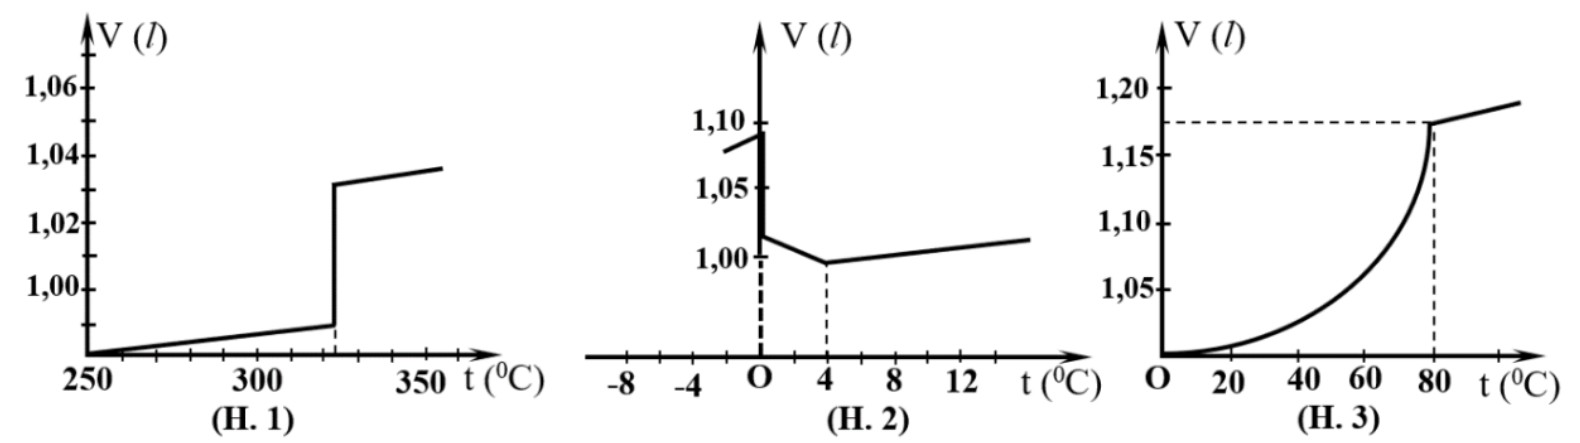
\includegraphics[scale=0.4]{figs/G12Y24B1-1}
	\end{center}
	\choiceTF[t]
	{Chì, nước đá và sáp nến đều có nhiệt độ nóng chảy tương ứng nhất định}
	{Trong quá trình nóng chảy của chì, nước đá và sáp nến thể tích của chúng đều tăng tỉ lệ thuận với nhiệt độ}
	{\True Trong quá trình nóng chảy, nhiệt độ của chì và nước đá không thay đổi, còn nhiệt độ của sáp thay đổi liên tục}
	{\True Khi nóng chảy, chì và sáp nến dãn nở (thể tích $V$ tăng) còn nước đá co lại (thể tích $V$ giảm)}
	\loigiai{}
\end{ex}
\subsection{BÀI TẬP TỰ LUẬN VÀ TRẢ LỜI NGẮN}
\setcounter{ex}{0}
\begin{ex}
	Hãy sử dụng mô hình động học phân tử để giải thích vì sao chúng ta có thể đi trong không khí, bơi trong nước nhưng không thể đi xuyên qua tường?
	\loigiai{
		Lực liên kết giữa các phân tử chất rắn lớn hơn nhiều so với lực liên kết giữa các phân tử chất lỏng và chất khí. Do đó, ta khó bẽ gãy được liên kết của các phân tử chất rắn nên không thể đi xuyên qua tường.
		
	}
	\end{ex}
%=====================================================================================
\begin{ex}
Cùng một chất, khi ở thể lỏng thường có khối lượng riêng nhỏ hơn khi ở thể rắn và khối lượng riêng ở thế khí lại nhỏ hơn khi ở thể lỏng. Vì sao như vậy?
	\loigiai{Vì khoảng cách trung bình giữa các phân tử chất khí lớn hơn khoảng cách trung bình giữa các phân tử chất lỏng và lớn hơn khoảng cách trung bình giữa các phân tử chất rắn. Do đó, với cùng một chất thì thể khí thường có thể tích lớn hơn so với với thể lỏng và lớn hớn thể tích ở rắn. Vì vậy, ở thể lỏng thường có khối lượng riêng nhỏ hơn khi ở thể rắn và khối lượng riêng ở thế khí lại nhỏ hơn khi ở thể lỏng.}
\begin{note}
Không đúng cho tất cả trường hợp. Ví dụ, nước có thể tích ở thể rắn lớn hơn thể tích ở thể lỏng
\end{note}
	\end{ex}
%=====================================================================================
\begin{ex}
Cồn y tế chuyển từ thể lỏng sang thể khí rất nhanh ở điều kiện thông thường. Hãy giải thích tại sao khi xoa cồn vào da, ta cảm thấy lạnh ở vùng da đó?
	\loigiai{
		Khi cồn chuyển thể từ lỏng sang khí thì cần thu nhiệt lượng, do đó tay ta mất bớt nhiệt lượng truyền cho cồn và cảm thấy vùng da thoa cồn bị lạnh đi.
		
	}
	\end{ex}

%=====================================================================================
\begin{ex}
	Để khử trùng các dụng cụ y tế nhiều lần (kéo, kẹp gắp, dao mổ, \dots), ngày nay người ta thường sấy chúng trong lò sấy ở nhiệt độ cao. Tuy nhiên, trước đây người ta thường phải luộc chúng trong nước sôi. Giả sử cần phải thực hiện nhiệm vụ này nhưng có một số vi khuẩn chỉ bị tiêu diệt ở nhiệt độ $\SI{105}{\celsius}$, trong đó khi nhiệt độ sôi của nước ở điều kiện tiêu chuẩn là $\SI{100}{\celsius}$. Hãy đề xuất phương án đơn giản để diệt các vi khuẩn này và giải thích.
	\loigiai{
		Tăng áp suất đun nước (dùng nối áp suất) để tăng nhiệt độ sôi của nước.
	}
\end{ex}
%=====================================================================================
\begin{ex}
Một người thợ mộc sau khi đánh vecni vào một số chân giường, sau một thời gian, người thợ mộc phát hiện thấy những chân giường chưa được đánh vecni bị nứt (rạn chân chim), còn những chân giường đã được đánh vecni thì không bị như thế. Hãy giải thích tại sao?
	\loigiai{
		Trong gỗ có chứa một lượng nước nhất định, khi đánh vecni lên gỗ, lớp vecni ngăn cách sự tiếp xúc của gỗ với môi trường bên ngoài và làm hạn chế sự bay hơi của nước trong gỗ. Còn những chân giường không đánh vecni thì nước trong gỗ bị bay hơi và làm gỗ bị khô, nứt.
	}
\end{ex}
% ===============================================================
\begin{ex}
	\immini{Hình bên là đồ thị biểu diễn sự phụ thuộc của nhiệt độ vào thời gian đun một ấm nước ở áp suất tiêu chuẩn. Nếu nhiệt lượng mà bếp tỏa ra không thay đổi trong suốt thời gian đun thì sau bao nhiêu giây kể từ lúc bắt đầu đun nước sẽ sôi?}{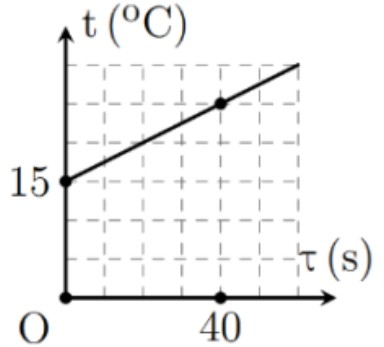
\includegraphics[scale=0.3]{figs/G12Y24B1-2}}
	\shortans[oly]{340}
	\loigiai{
		\SI{340}{\second}.
	}
\end{ex}
% ===============================================================
\begin{ex}
	\immini{Bằng các nghiên cứu, người ta phát hiện ra rằng các nguyên tử của nguyên tố X sắp xếp tuần hoàn tạo thành mạng tinh thể gồm các ô hình lập phương giống hệt nhau xếp chồng lên nhau (Hình a). Ở mỗi ô lập phương nhỏ nhất (gọi là ô mạng cơ sở) có một nguyên tử nằm tại tâm và ở mỗi đỉnh của nó đều có một nguyên tử (Hình b). Biết rằng chiều dài cạnh của mỗi ô lập phương cơ sở là $a=\SI{2.87E-10}{\meter}$. Biết khối lượng mỗi nguyên tử X là \SI{9.3E-26}{\kilogram}. Khối lượng riêng của nguyên tố X là bao nhiêu \si{\kilogram/\meter^3}? (Chỉ lấy phần nguyên của kết quả).}{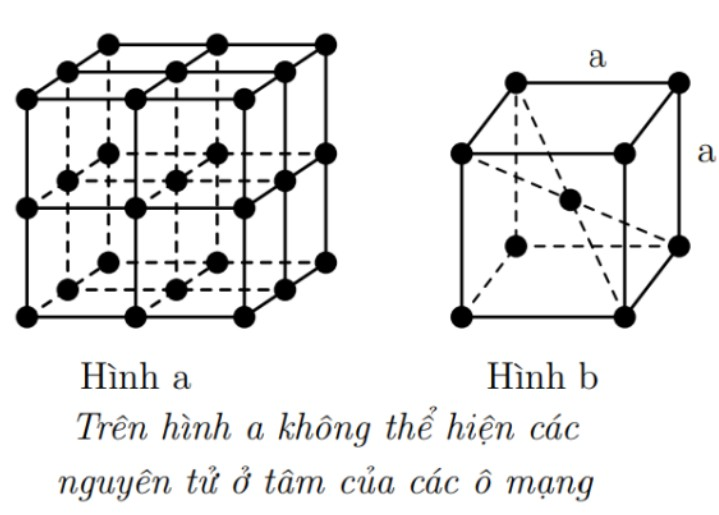
\includegraphics[scale=0.4]{figs/G12Y24B1-3}}
	\shortans[oly]{7868}
		\loigiai{
			Mỗi ô mạng có thể tích là $a^3$ gồm:
			\begin{itemize}
				\item 8 nguyên tử ở đỉnh, mỗi nguyên tử chỉ đóng góp 1/8 cho ô mạng;
				\item 1 nguyên tử ở tâm.
			\end{itemize}
			$\Rightarrow$ tổng đóng góp cho 1 ô mạng là $8\cdot\dfrac{1}{8}+1=2$ nguyên tử.
			$$D=\dfrac{m}{V}=\dfrac{2\cdot m}{a^3}\approx\SI{7868}{\kilogram/\meter^3}.$$
		}
	\end{ex}
